\section{Le contexte}
\paragraph{}
Project for ``PJI''... but also for Bachelor's Thesis\\
At the time working at this project, 5 semesters as a student at... last semester erasmus student...\\

\section{L'idée}
TL;DR: Eye tracking using computer's webcam; move cursor with eyes.\\

\section{Motivation}
\paragraph{}
I wanted a project that would help me learn... related to... (AI, ML) because I want to have a carreer as an...\\
Also, I was deeply motivated by doing something that could actually be used as a practical tool... or help anybody in a way...\\
Wanted to work on a series of experiments with MLPs, CNNs... in order to learn...\\

\paragraph{}
Question: Is it wrong to place images in the "introduction" chapter?

\section{Le but}

\subsection{Objectifs essentiels}
\paragraph{}
Cross-platform app\\
Base functionality: predict where the user's looking on a grid 3x3. Based on the grid, we can "artifficially" move the cursor.
\begin{figure}[H]
    \centering
    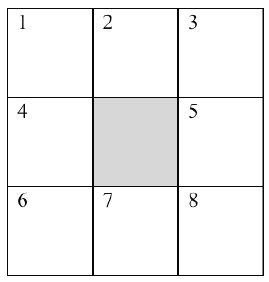
\includegraphics[width=100pt]{3x3_grid.png}
    \caption{3x3 Grid}
    \label{}
\end{figure}
\paragraph{}
Looking at square $2$ will move the cursor up by $dy$. Looking at square $6$ will move it to the bottom-left by $dx$ and $dy$ and so on.
\\

App easy to maintain: use concepts learn throughout university: classes, cohesion, SOLID principles\\
*to mention that Python isn't exactly the best language to take OOP into consideration, but use OOP more like general guidelines
\\

Left click = long blink with left eye, right click = long blink with right eye


\subsection{Objectifs préférables}
\paragraph{}
If predicting the squares works well, try regression: try to predict the exact position of the cursor
\\

Maybe find a way to click without using hands: maybe recognize when the user \emph{says} ``click''?
\\